\documentclass{article}
\usepackage{tikz}
\usetikzlibrary{shapes}
\begin{document}
\begin{center}
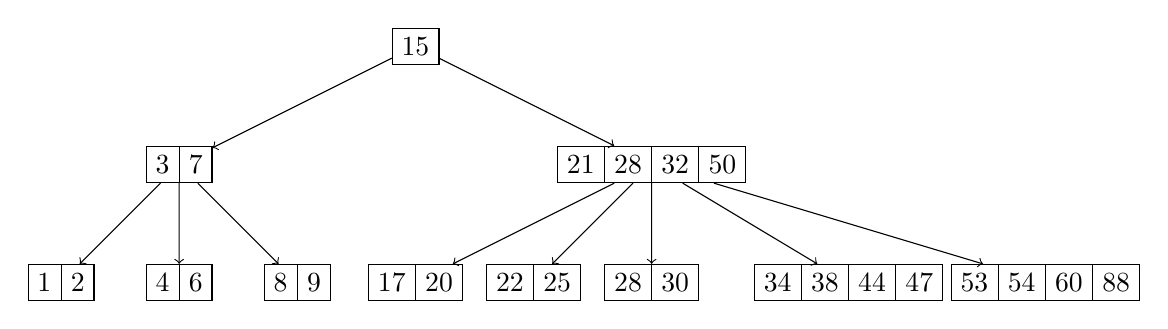
\begin{tikzpicture}
\tikzstyle{bplus}=[rectangle split, rectangle split horizontal,rectangle split ignore empty parts,draw]
\tikzstyle{every node}=[bplus]
\tikzstyle{level 1}=[sibling distance=60mm]
\tikzstyle{level 2}=[sibling distance=15mm]
\node {15} [->]
  child {node {3 \nodepart{two} 7}
    child {node {1 \nodepart{two} 2}}
    child {node {4 \nodepart{two} 6}}
    child {node {8 \nodepart{two} 9}}    
  } 
  child {node {21 \nodepart{two} 28 \nodepart{three} 32 \nodepart{four} 50}
    child {node {17 \nodepart{two} 20}}
    child {node {22 \nodepart{two} 25}}
    child {node {28 \nodepart{two} 30}}    
    child[sibling distance=25mm] {node {34 \nodepart{two} 38 \nodepart{three} 44 \nodepart{four} 47}}    
    child[sibling distance=25mm] {node {53 \nodepart{two} 54 \nodepart{three} 60 \nodepart{four} 88}}    
  }
;\end{tikzpicture}
\end{center}

\end{document}